\section{Actor basierte Architekturmuster}\label{sec:theory:actorArchitecture}
Die Entwicklung von gängigen Designmustern wie beispielsweise jene der \textit{Game of Four} (siehe \cite{gangOfFour1995design}), sind auf die Objektorientierte Programmierung ausgerichtet. Im \textit{Actor Model} können eine vielzahl dieser Muster nicht mehr verwendet werden bzw. ihre stärken nicht mehr optimal ausspielen. Um die stärken des \textit{Actor Models} optimal auszuspielen sind etliche Architekturmuster entstanden, welche unter anderem in \cite{Vernon2015ReactiveAkka} und \cite{kuhn2017reactive} beschrieben werden. Einige dieser Muster werden nachfolgend beschrieben um die Verständlichkeit mit der Arbeit des \textit{Actor Models} zu erhöhen.

\subsection{Request-Replay}
Das einfachste, und gleichzeitig wohl wichtigste Muster innerhalb des \textit{Atore-Models} ist das \textit{Request-Replay} Muster. Es wird benötigt Inhalte von einem Actor abzufragen. Wie in \ref{actor:requirements:shareNothing} beschrieben, darf ein Actor keine Informationen nach außen geben. Möchte nun ein Actor Informationen von einem anderen Actor haben, so muss dieser eine Nachricht an den betroffenden Actor senden, dieser sendet dann eine neue Nachricht, mit den entsprechenden Informationen, an den anfragenden Actor zurück. Die Antwort Nachricht kommt dabei nicht als direkte Antwort der Nachricht, sondern als eigenständige Nachricht an den fragenden Actor zurück. Es wird zwar von der Antwort gesprochen, wie jedoch in \ref{actor:requirements:AsynchronCommunication} beschrieben ist jede Anfrage an einen Actor asynchron. Deshalb wird die Antwort wieder in die Mailbox des Empfängers zugesendet. Zur vereinfachung wird jedoch von einer Antwort Nachricht gesprochen. \\
In der Abbildung \ref{fig:actor:patterns:requestReplay} ist das \textit{Request-Replay} abgebildet. Der Actor \textit{A} sendet eine \textit{Command-Message} an den Actor \textit{B}, dieser Verarbeitet diese Nachricht, und sendet eine neue \textit{Document-Message} zurück an Actor \textit{A}. Somit kann Actor \textit{A} mit den Informationen von Actor \textit{B} weiterarbeiten.  \\
Dieses Pattern gilt als Grundlage für die alle weiteren Patterns und veranschaulicht das Prinzip eines typischen Workflows in einem Actor System. \citep{Vernon2015ReactiveAkka}
\begin{figure}
    \centering
    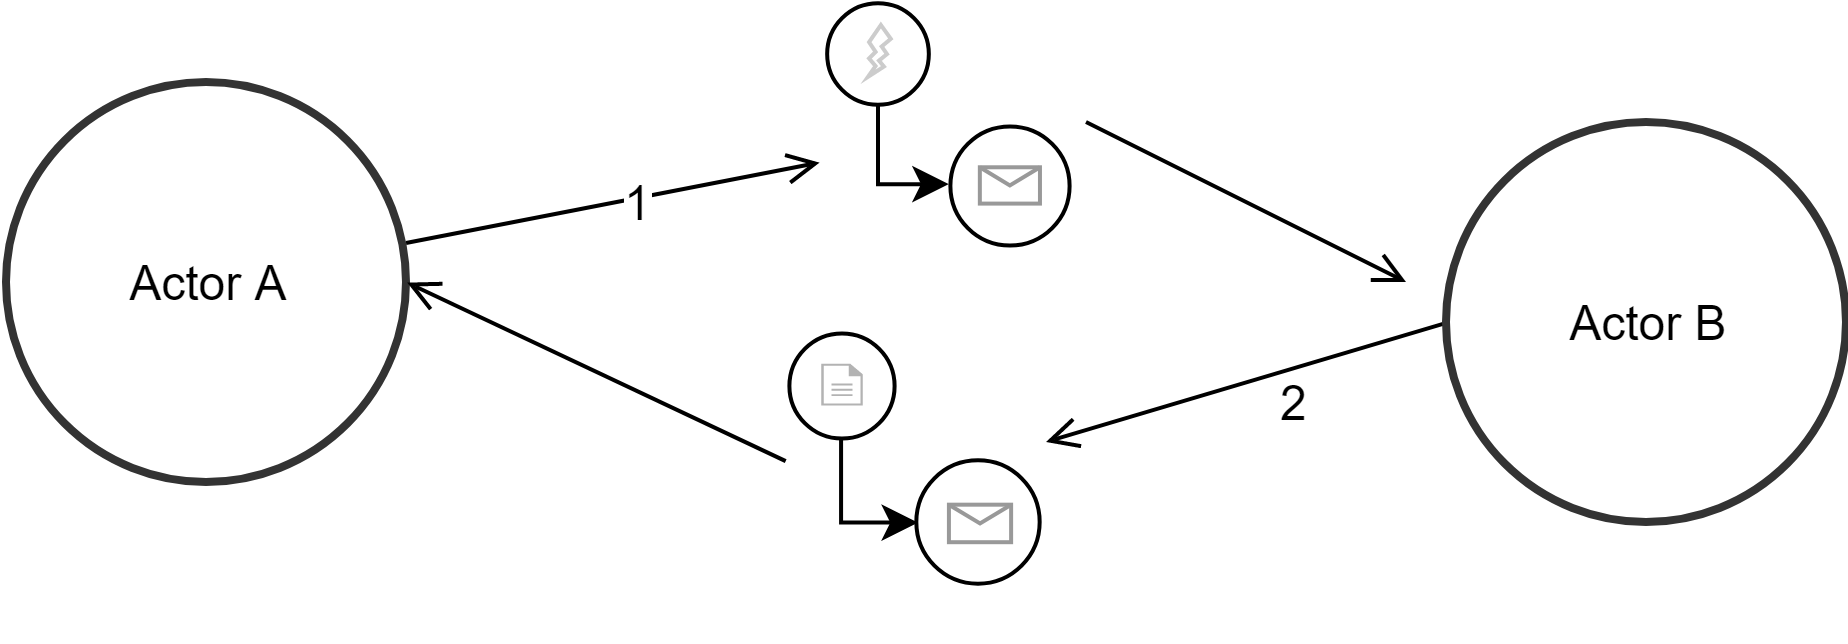
\includegraphics[width=\linewidth]{gfx/actor/patterns/requestReplay}
    \caption{Das \textit{Request-Replay} Pattern}
    \label{fig:actor:patterns:requestReplay}
\end{figure}

% todo correlation identifier erklären

\subsection{Return Adress}
Damit ein Actor eine Nachricht an einen anderen Actor senden kann, benötigt er wie in \ref{sec:actors:messages} erklärt, eine Adresse dessen. Diese kann auch in einer bereits empfangenen Nachricht enthalten sein. \\
In Abbildung \ref{fig:actor:patterns:returnAdress} ist zu sehen, dass ein Actor ein \textit{Command} and einen anderen Actor sendet, und diesen \textit{Command} Anweist die Antwort an einen anderen Actor zu senden. \\
Diese somit bekannt gegebene Adresse könnte auch für zukünftige Verarbeitungen von Nachrichten verwendet werden. In \cite{Vernon2015ReactiveAkka} wird beispielsweise ein Server/Client Prinzip zwischen Actors besprochen. Der Client-Actor bekommt dann zu Beginn seines Lebenszyklus die Adresse eines Server-Actors übermittelt. Alle Informationen die der Client im weiteren Verlauf erarbeitet, werden dann an den Server übermittelt.

\begin{figure}
    \centering
    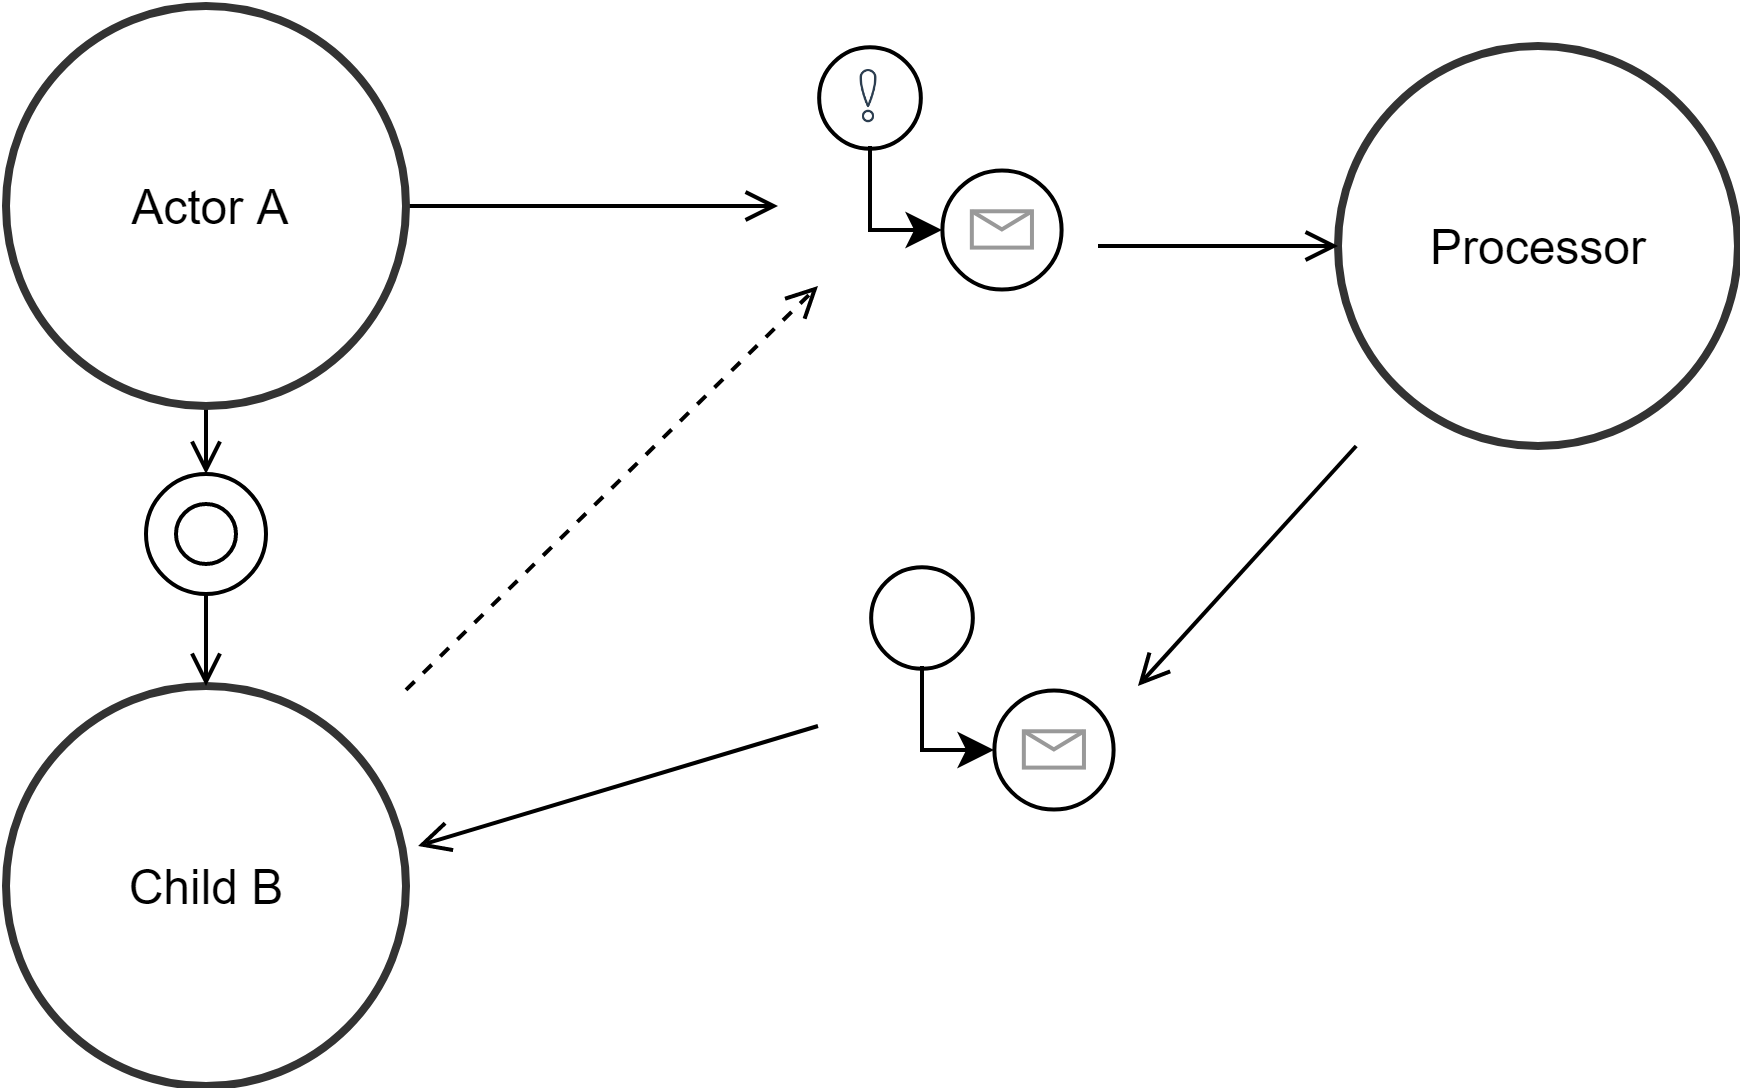
\includegraphics[width=\linewidth]{gfx/actor/patterns/returnAddress}
    \caption{Der Processor empfängt von Actor A ein Kommando. Die Nachricht enthält jedoch die Information, das Ergebnisse nicht an den Absender zu senden sind, sondern an den Actor B.}
    \label{fig:actor:patterns:returnAdress}
\end{figure}


\subsection{Processor}\label{sub:actor:patterns:processor}
Eine Möglichkeit komplexe Prozesse mit dem Actor-Model abzubilden, ist ein \textit{Processor}-Actor. Dieser koordiniert, abgestimmt auf einen bestimmen Geschäftsprozess, alle Vorgänge und liefert, falls gewünscht, abschließend oder periodisch ein Ergebnis zurück. Es gibt verschiedenste Varianten von \textit{Processor}-Actoren. \citep{Vernon2015ReactiveAkka}
Oft verwenden \textit{Processors} auch \textit{Router} (siehe \ref{sec:actor:patterns:routing}) und \textit{Aggregatoren} (siehe \ref{sec:actor:patterns:aggregator}) um Ihren Prozesse in einem Actor-System abzubilden. \\
Ein Typisches Beispiel kann in Form eines Bestellprozesses gezeigt werden. Im Ablauf des schemenhaft gezeigten \textit{Order Processors} in Abbildung \ref{fig:actor:patterns:orderProcesseor} sind drei andere Komponenten, welche hier als Actors dargestellt werden, beteiligt. Der Statistik Actor sowie die zwei \textit{Inventories} können sich auch aus mehreren Actors formieren, ist jedoch für den \textit{Order-Processor} nicht relevant. Vielmehr, ist der \textit{Processor} in diesem Fall Verantwortlich den Bestellprozesses vollständig auszuführen, in dem er die Beteiligten Actors über den Vorgang Informiert bzw. weitere Kommandos an diesen abgibt. Sind alle erforderlichen Antworten eingetroffen, kann er die Bestellung abschließen und dies wiederum über eine \textit{Event}-Nachricht an den Besteller signalisieren. \\
In diesem Beispiel fungiert der \textit{Processor} auch als \textit{Aggregator}, da er auf mehrere Nachrichten wartet, und anhand dieser eine Antwort generiert. 

\begin{figure}
    \centering
    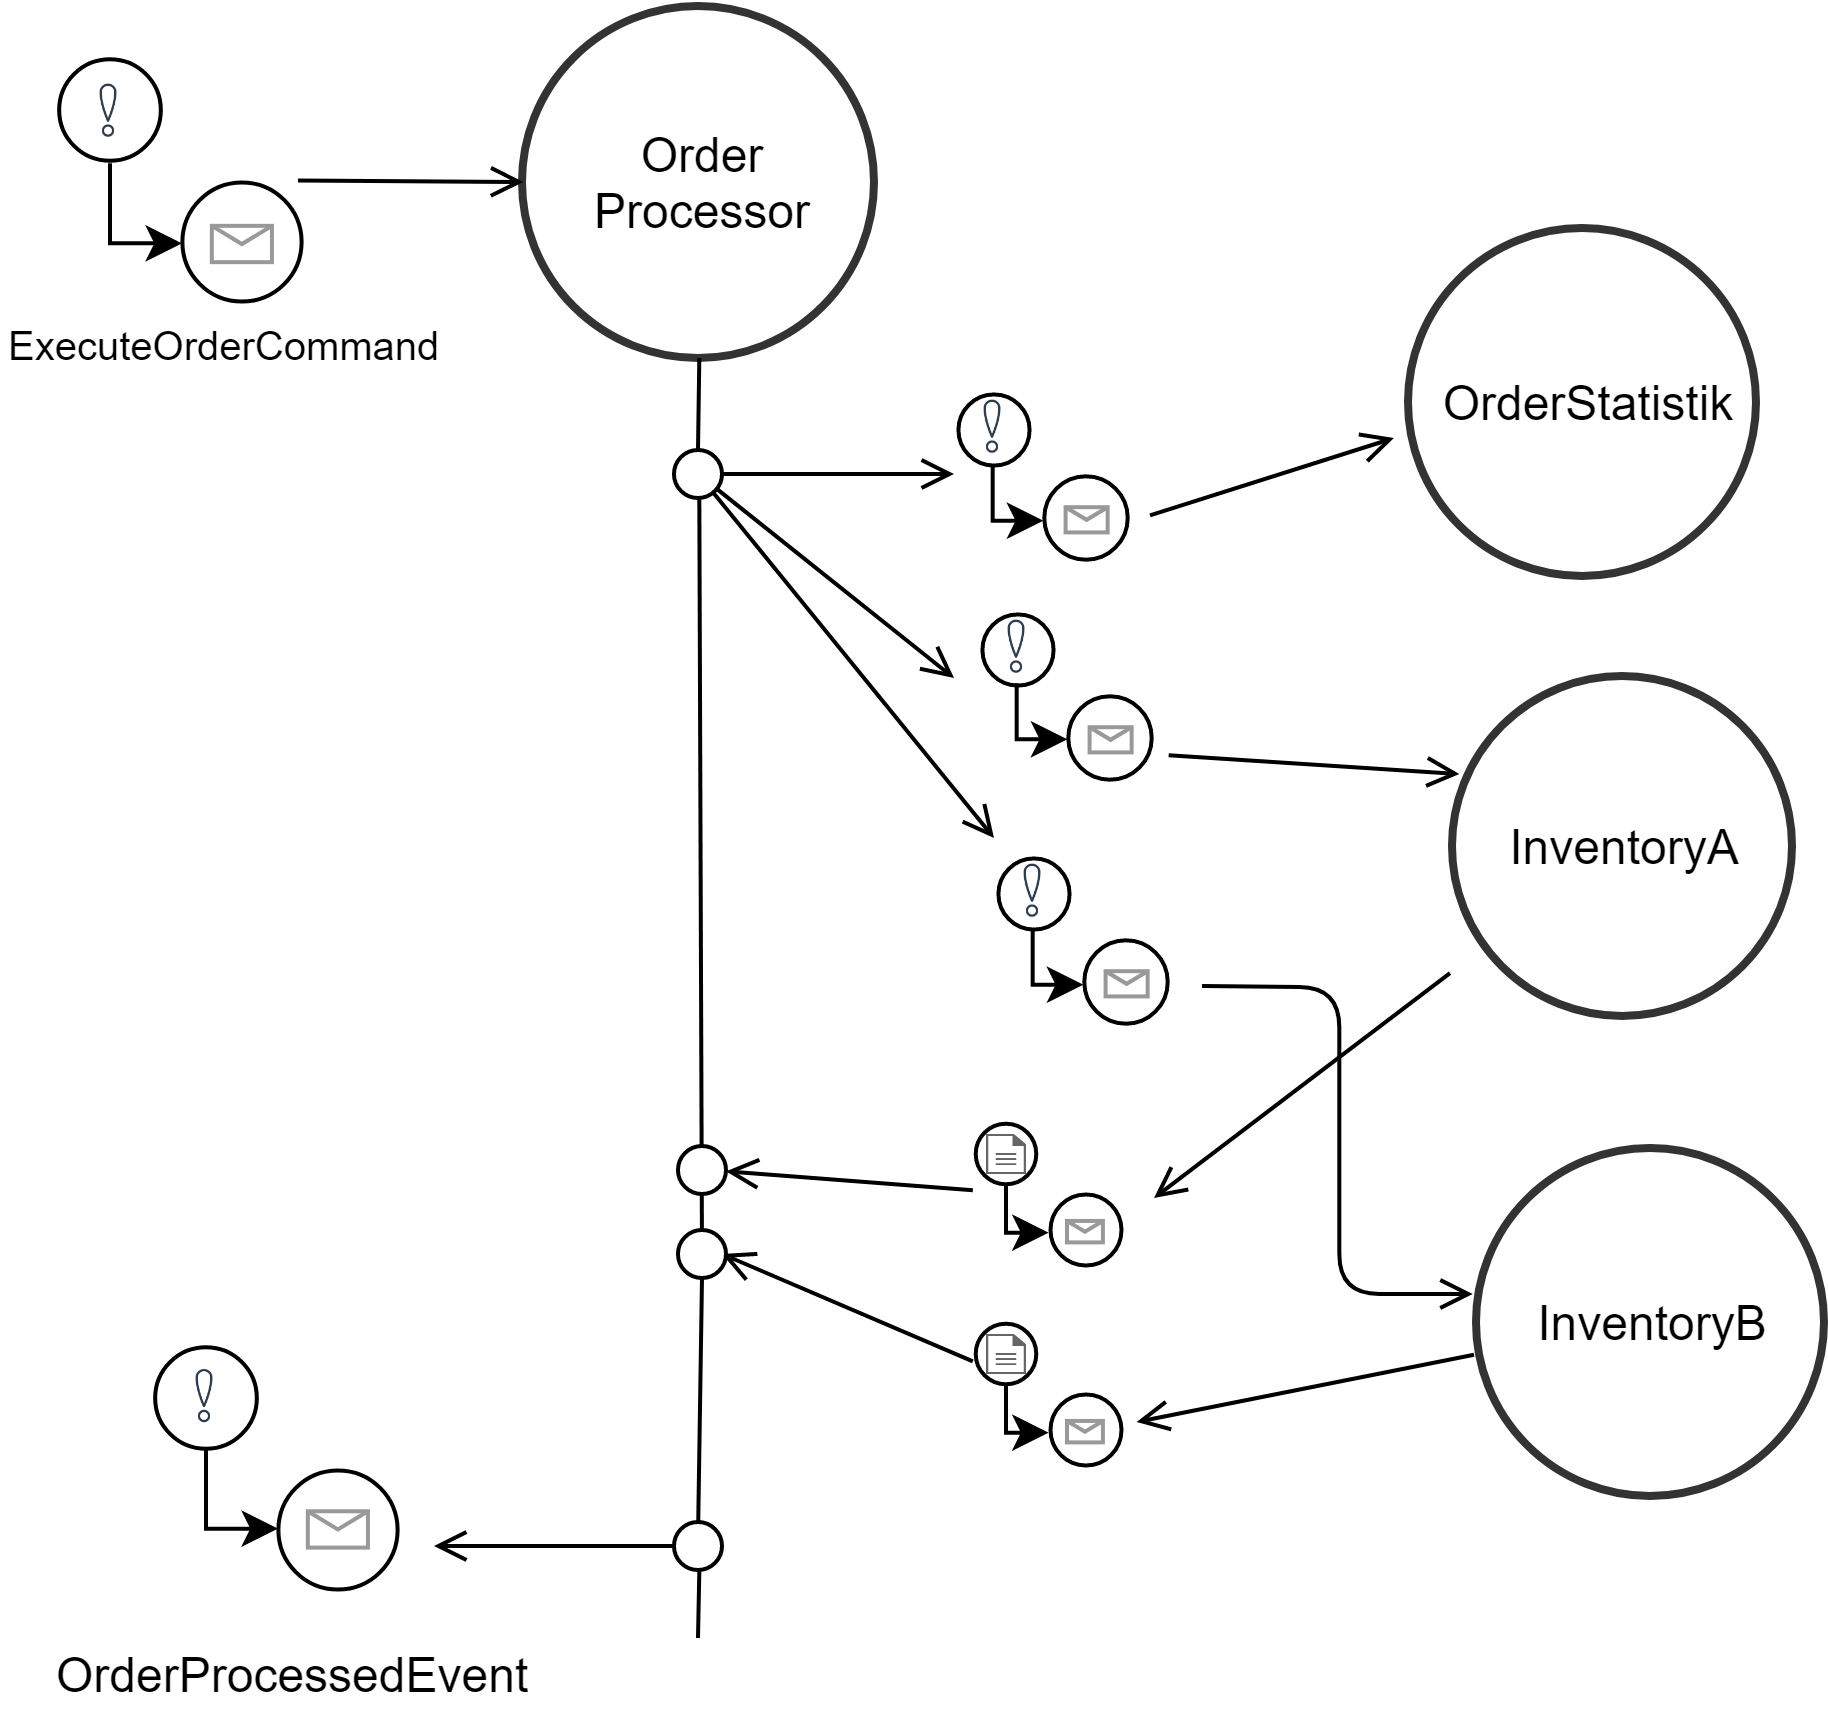
\includegraphics[width=0.9\linewidth]{gfx/actor/patterns/simpleOrderProcesor}
    \caption{Ein schemenhafter Bestellprozess welcher mehrere andere Actors miteinbezieht.}
    \label{fig:actor:patterns:orderProcesseor}
\end{figure}

\subsection{Routing}\label{sec:actor:patterns:routing}
In einem Actor System versteht man laut \cite{Vernon2015ReactiveAkka} und \cite{kuhn2017reactive} eine Komponente, welche ankommende Nachrichten an einen oder mehrere Actors weitersendet. \\
In \cite{Vernon2015ReactiveAkka} sind eine vielzahl an unterschiedlichsten Routern beschrieben. Wie die meisten anderen Komponenten auch, ist ein Router ein Actor. Dieser Actor bekommt dann die Aufgabe einkommende Nachrichten entsprechend weiterzuleiten. Dazu kann ein Router verschiedene Faktoren für das Routing einbeziehen. Als Beispiel ist unter anderem zu nennen, dass, der Router Informationen aus der Nachricht entnimmt, und anhand dieser das Routing vornimmt. Weiters können auch Einflüsse des Actor-System einbezogen werden. In \cite{Vernon2015ReactiveAkka} und \cite{Akka.netCommunityAkka.NETDocumentation} ist zu lesen, das ein Router CPU oder Speicherauslastung von verschiedenen Systemen überwacht, und neue Nachrichten an das am wenigsten ausgelastete System zukommen lässt. \\
\cite{Vernon2015ReactiveAkka} kategorisiert Router in folgende drei Kategorien. 
\begin{description}
    \item[Einfache Router] Werden Nachrichten von einem Actor an einen anderen Actor weitergeleitet spricht man von einem einfachen Router. Diese Router leiten Nachrichten anhand des Inhaltes oder anderen Faktoren an andere Actors weiter. Weiters ist es auch möglich das ein Router eine einzelne Nachricht in mehrere Nachrichten aufteilt, und diese dann einzeln an andere Actoren weiterleitet. Die Möglichkeiten von Routern ist umfangreich und daher gibt es unzählig verschiedene.
    \item[Zusammengesetzte Router] Da einfache Router nur exakt eine einzige Aufgabe vollführen, können für komplexere Aufgaben mehrere einfache Router zusammen verwendet werden und bilden dann einen zusammengesetzten Router. Für den verwender eines zusammengesetzten Routers spielt es jedoch keine Rolle welche einfachen Router dafür verwendet werden.
    \item[Architektonische Router] Um die Entkoppelung von Komponenten und Actoren zu ermöglichen, können Router eingesetzt werden, dessen Aufgabe es ist diese Entkoppelung zu erwirken. Sie werden zwar nicht für den konkreten Ablauf eines Prozesses benötigt, bewirken jedoch Verbesserungen beim Durchsatz und der Erweiterbarkeit. 
\end{description}
Durch den Einsatz von Routern können Prozesse und Abläufe durch Actors abgebildet werden und eine optimale, an das Aufgabengebiet angepasste Verteilung erwirkte werden. Die in \cite{Vernon2015ReactiveAkka} diskutierten Router Beispiele zeigen auf, welche Vielzahl an Einsatzmöglichkeiten ein Actor als Router ermöglichen kann. 

\subsection{Aggregator}\label{sec:actor:patterns:aggregator}
Wie bereits im Beispiel in Kapitel \ref{sub:actor:patterns:processor} gezeigt, kann ein Actor die Aufgabe haben, auf verschiedene Nachrichten zu warten, um abschließend eine Antwort zu erstellen und zu versenden. Der Actor aggregiert somit eine beliebige Anzahl an Nachrichten und erzeugt daraus neue Nachrichten. \\
Der Aggregator kann durch folgende, in \cite{Vernon2015ReactiveAkka} gelisteten Kriterien, erkennen wann die Aggregation abgeschlossen ist.
\begin{itemize}
    \item Alle zu erwartenden Nachrichten sind eingetroffen
    \item Zeitfenster ist abgelaufen
    \item Nachricht mit optimalen Kriterien eingetroffen
    \item Ein externes Event ist eingetreten
    \item Ablauf eines Zeitfensters oder eines der anderen vier Kriterien
\end{itemize}
Welches der fünf Kriterien ein Aggregator für die Terminierung verwendet, hängt stark von der eigentlichen Aufgabe ab. Ein Aggregator selber kann, wie in \cite{Vernon2015ReactiveAkka} beschrieben, auch als Router fungieren, dies ist jedoch nicht zwingend erforderlich.

\subsection{Garantierte Nachrichtenzustellung}
Die Zustellung von Nachrichten zu einem Actor unterliegt allgemein keiner Garantie das sie dort auch ankommt, geschweige den Verarbeitet wird. Schon in \cite{Agha1985ConcurrentParallelism} wird dieses Problem skiziert. Auch \cite{Vernon2015ReactiveAkka} oder \cite{CloudComputingPatterns2014} verweisen auf dieses Problem das nicht gewährleistet werden kann, das eine Nachricht an einen Actor auch ankommt. In \cite{CloudComputingPatterns2014} generalisiert dieses Problem das Nachrichten zwischen Komponenten generell keiner garantierten Zustellung unterliegen. \\
Um in einem solchen System jedoch die Zustellung von Nachrichten zu gewährleisten gibt es Muster welche die Zustellung einer Nachricht überwachen. In \cite{messagedeliveryreliabilityakkadocumentation} sowie \cite{hughmckee_2017} werden drei Kategorien für die Zustellung von Nachrichten genannt.
\begin{description}
    \item [Höchstens einmal] Eine Nachricht wird entweder garnicht oder maximal einmal zugestellt. Diese Kategorie wird erreicht, wenn eine Nachricht ohne spezielle vorkehrungen an einen Actor gesendet wird. Sie kommt entweder an, oder sie geht verloren.
    \item [Mindestens einmal] Die Nachricht wird mindestens einmal oder beliebig oft zugestellt. Die Nachricht wird so oft verwendet, bis eine Bestätigung eintrifft. Das führt jedoch zu dem Umstand, falls die Bestätigung während der Zustellung verloren geht, auch die Nachricht selbst öfters zugestellt werden kann.
    \item [Exakt einmal] Die Nachricht wird exakt einmal zugestellt. Erfordert jedoch viele Ressourcen und ist nur schwer Realisierbar.
\end{description}
\cite{Vernon2015ReactiveAkka} zeigt eine variante der garantierten Nachrichtenzustellung mit dem \textit{Actor-Model}, welche die zustellung mindestens einmal garantiert. Dabei wird beim versenden die gesendete Nachricht in einem permantenten Speicher abgespeichert. Trifft die Bestätigung der gesendeten Nachricht ein, wird die gespeicherte Nachricht entsprechend markiert. Vergeht nach dem versenden der Nachricht ein definiertes Zeitfenster ohne eintreffen einer Bestätigung, so wird die Nachricht erneut versendet. Dies geschieht solange bis die Bestätigung einlangt. \\
Generell ist jedoch immer zu beachten, das das versenden einer Nachricht fehlschlagen kann. Je nach Anwendungsfall muss dies vom Entwickler beachtet werden, und entsprechende Maßnahmen dafür getroffen werden. Die Gründe weshalb eine Nachricht nicht Ordnungsgemäß zugestellt wird sind zahlreich. So kann beispielsweise die Nachricht über ein Netzwerk gesendet werden und somit kann auch das Paket verloren gehen. Weiters ist es möglich, das der Empfänger der Nachricht nicht reagiert weil die Mailbox voll ist oder der Prozess welchen den Empfänger beherbergt nicht reagiert. Die Gründe für die Unzustellbarkeit sind zahllos, weshalb die Zustellbarkeit auch nicht garantiert werden kann. \citep{messagedeliveryreliabilityakkadocumentation}







 